%Template da SBC para artigos em português

\documentclass[12pt]{article}

%\usepackage{hyperref}
\usepackage{xcolor}
\usepackage{sbc-template}
\usepackage{graphicx,url}
\usepackage[utf8]{inputenc}
\usepackage[brazil]{babel}
%\usepackage[latin1]{inputenc}

\newcommand*{\captionsource}[2]{%
  \caption[{#1}]{#1}\par
  \textbf{Fonte:} #2\par
}


\sloppy

\title{Instructions for Authors of SBC Conferences\\ Papers and Abstracts}

\author{Gabriel Lando\inst{1}, Juliano Wickboldt\inst{1}}


\address{Instituto de Informática -- Universidade Federal do Rio Grande do Sul
  (UFRGS)\\
  Caixa Postal 15.064 -- 91.501-970 -- Porto Alegre -- RS -- Brazil
  \email{\{glando, jwickboldt\}@inf.ufrgs.br}
}

\begin{document} 

\maketitle

\begin{abstract}
With the advent of the fifth generation of mobile networks, new functionalities were adde, making these networks increasingly complex.
The increase in the processing capacity of general-purpose processors allowed the cores of mobile networks to run in software, reducing the deployment costs of these networks, but making them more susceptible to implementation errors.
This work carries out a literature review bringing the advances of mobile networks from its beginning to the fifth generation, making a survey on tests in open source implementations of mobile networks core.
Finally, a method is proposed to test the performance of some implementations of mobile networks core form the fifth generation in order to evaluate the behavior of these implementations under heavy workload.
\end{abstract}
     
\begin{resumo} 
Com o advento da quinta geração de redes móveis, novas funcionalidades foram adicionadas tornando as redes cada vez mais complexas.
O aumento da capacidade dos processadores de propósito geral permitiram que os núcleos de redes móveis pudessem ser executados em software, reduzindo-se os custos de implantação dessas redes. Conteúdo, isso também tornou-as mais suscetíveis a erros de implementação e problemas de desempenho.
Este trabalho realiza uma revisão da literatura trazendo os avanços das redes móveis desde o seu princípio até a quinta geração, fazendo um levantamento sobre testes em núcleos de redes móveis que possuem implementação em código aberto.
Por fim, é proposto um método para testar o desempenho de algumas implementações de núcleos da quinta geração de redes móveis com o intuito de avaliar o comportamento dessas implementações sob alta carga de trabalho.

\end{resumo}

\section{Introdução}
A quinta geração de redes móveis (5G) teve sua especificação inicial disponibilizada em 2017 na \textit{Release 15} da 3GPP \cite{Redana2020}, trazendo diversas melhorias em relação a quarta geração (4G). \textcolor{red}{QUAIS SÃO AS MELHORIAS? }
É possível citar como principais metas do 5G em relação às gerações anteriores maiores taxas de transferência de dados, maior área de cobertura e menor latência de comunicação \cite{Ahmad2019}.
\textbf{TODO: ADICIONAR MAIS ALGUMA COISA} 

Para que seja possível atingir as metas propostas, uma evolução no núcleo da rede se torna necessária por ser considerado o elemento mais crítico do 5G \cite{Cardoso2020}. 

\textbf{(no mínimo 3 frases por paragrafo)}

\textbf{Escrever sobre 5G geral}

\textbf{Desempenho do 5G}

\textbf{5G em software}

\textbf{Software sem garantias (é preciso testar).}

O conceito de redes móveis privadas surgiu com o advento da Indústria 4.0, que visa transformar a manufatura industrial por meio da digitalização e exploração das potencialidades das novas tecnologias \cite{Rojko2017}.
Uma indústria pode criar e gerenciar sua própria rede 4G ou 5G, permitindo a conexão de milhares de dispositivos e sensores, provendo segurança, performance e baixa latência.
Existem implementações \textit{open source} de estações de rádio e núcleos de redes 4G e 5G disponíveis, como \textit{free5GC}\footnote{\url{https://www.free5gc.org}}, \textit{Open5GS}\footnote{\url{https://open5gs.org}}, \textit{OpenAirInterface}\footnote{\url{https://openairinterface.org}} (OAI), \textit{srsRAN}\footnote{\url{https://www.srslte.com}}, dentre outras, facilitando a implantação desse tipo de rede móvel em ambientes corporativos.

Uma vez que deseja-se implantar uma rede móvel privada, é preciso avaliar o cenário para que possa ser feita a implementação com a melhor relação custo-benefício possível.
Sendo assim, é preciso avaliar, principalmente, a área de cobertura a ser atendida pelas antenas, quantos dispositivos serão conectados, qual o tráfego de dados que será gerado e qual a latência máxima desejada para a comunicação dos dispositivos.
Após coletar essas informações, pode-se definir o tipo de equipamento que precisa ser adquirido para suprir a necessidade dessa rede.
Entretanto, para que se possa definir qual o \textit{hardware} a ser usado, é preciso saber como as implementações \textit{open source} se comportam ao serem executadas nesses equipamentos.

Nesse contexto, estão inseridos os testes para averiguar o comportamento dessas redes móveis em diversos cenários.
Como as implementações \textit{open source} não possuem garantias, é preciso executar testes de conformidade e robustez, por exemplo para garantir que o núcleo da rede se comporte da forma que foi especificado.
Além disso, é preciso aferir o desempenho das diversas implementações, permitindo com que seja possível avaliar qual \textit{hardware} seria capaz de rodar a implementação desejada de acordo com a capacidade da rede que se deseja implantar.

Desta forma, o presente trabalho tem como objetivo responder a seguinte questão: como se comportam as diferentes implementações \textit{open source} de core 5G para execução dos procedimentos em escala?


\section{\textit{Background}} \label{sec:background}
\subsection{Antes do 5G}

Quando se trata de redes móveis, é importante analisar a evolução dessa tecnologia. Originalmente, as redes móveis tinham o foco em comunicações de voz analógica, sendo uma extensão da rede de telefonia pública \textit{(Public Switched Telephone Network - PSTN)}, que operava com rede de roteamento de circuitos \cite{Cardoso2020}.
Entretanto, essas redes móveis foram adaptadas para transporte de dados com taxas de transmissão muito baixas, sendo conhecida como rede móvel de primeira geração (1G).

Com a necessidade de evoluir as redes 1G, surge a segunda geração (2G), que provia um sinal com melhor qualidade, maiores taxas de transferência de dados e maior aproveitamento do espectro das ondas de rádio.
Todavia, essa tecnologia ainda mantinha seu foco em roteamento de circuitos.
Nessa geração, também surge o serviço de troca de mensagens curtas, conhecido como \textit{Short Message Service} (SMS).
Foi no 2G que a tecnologia de transporte de dados \textit{Global System for Mobile Communications} (GSM) foi inserida.
\textcolor{red}{\textbf{ToDo: citar artigo sobre.}}

Em 1998, inicia-se a parceria entre diversas organizações responsáveis pela criação dos padrões de telecomunicação denominada \textit{3rd Generation Partnership Project} (3GPP)\footnote{\url{https://www.3gpp.org/about-3gpp}} que publica a \textit{Release 1999} no início do ano 2000.
Essa \textit{release} descreve uma nova tecnologia de redes móveis, com foco em roteamento de pacotes.
Porém, essa tecnologia mantinha a compatibilidade com as tecnologias antigas, sendo denominada de 3G, ou redes móveis de terceira geração \cite{release19993gpp}.

Ao final de 2008, a \textit{Release 8} é publicada pela 3GPP, especificando os requisitos para a tecnologia \textit{Long Term Evolution} (LTE), que viria para ser o substituto da terceira geração de redes móveis.
Entretanto, essa especificação não preenchia os requisitos mínimos para ser considerada a quarta geração de redes móveis, sendo assim conhecida como 3.9G \cite{delperal2018}.
Dentre as mudanças provindas desta nova tecnologia, é importante mencionar a remoção do suporte à roteamento de circuitos, fazendo com que essa geração usasse apenas roteamento de pacotes sobre IP para todo o tráfego de informações na rede.

Toda a informação de áudio de ligações telefônicas era trafegada sobre a rede de roteamento de circuitos nas gerações anteriores ao LTE.
Com a remoção dessa tecnologia no LTE, foi necessário desenvolver um novo protocolo para trafegar essas informações, surgindo assim o \textit{Voice over LTE} (VoLTE).
O VoLTE, assim como a tecnologia \textit{Voice over IP} (VoIP), trafega os dados de voz de ligações telefônicas sobre a rede de roteamento de pacotes, permitindo que as operadoras móveis pudessem continuar oferecendo o serviço de ligações telefônicas para seus clientes. Nesta época, esse serviço era o mais rentável para as operadoras \cite{Yi2012}. 

Visando preencher os requisitos mínimos para a criação da quarta geração de redes móveis (4G), no início de 2011 é publicada a \textit{Release 10} pela 3GPP, criando assim a tecnologia \textit{LTE-Advanced} (LTE-A) \cite{release103gpp}.
O 4G prometia velocidades de \textit{download} de pico de até 1Gbps e velocidades de \textit{upload} de pico de até 100Mbps.
Atingir tais velocidades só era possível graças à remoção do suporte ao roteamento de circuitos que ocorreu no 3.9G.

Antes do surgimento do LTE, existiam apenas 3 componentes na rede. Um era o equipamento de usuário, denominado \textit{User Equipment} (UE), sendo esse o dispositivo móvel. Outro componente era a estação de rádio base, ou \textit{Radio Access Network} (RAN), denominada na tecnologia 3G de \textit{UMTS Terrestial Radio Network} (UTRAN). Por fim, o núcleo da rede, ou \textit{Core Network} (CN), que no 3G era denominado \textit{UMTS Core Network} \cite{Miah2002}.
No entanto, a especificação da rede LTE trouxe uma melhor separação dos seus componentes do núcleo da rede, denominado \textit{Evolved Packet Core} (EPC) nessa geração.
O EPC foi separado em 4 componentes, sendo eles o \textit{Serving Gateway (Serving GW)}, o \textit{PDN Gateway (PDN GW)}, o \textit{Mobility Management Entity} (MME) e o \textit{Home Subscriber Server} (HSS) \cite{epc3gpp}.

\subsection{Redes 5G}

Em 2017, a 3GPP publica a versão inicial da \textit{Release 15}, com as definições da quinta geração de redes móveis, o 5G \cite{release153gpp}.
Assim como nas gerações anteriores, o 5G trouxe melhorias na capacidade de transmissão de dados da RAN e redução da latência de comunicação entre o UE e a RAN.
Entretanto, essa geração teve como objetivo criar uma rede mais dinâmica e com maior flexibilidade em relação ao LTE.
Nessa geração também houve a integração com tecnologias de comunicação sem fios não-3GPP, que enquadram dispositivos denominados de \textit{Internet of Things} (IoT).

A \textit{Release 15} também introduziu as arquiteturas de rede 5G \textit{Non-Stand  Alone} (NSA) e 5G \textit{Stand Alone} (SA).
Na arquitetura NSA, o núcleo da rede 4G é utilizado para a autenticação e comunicação dos dispositivos 5G, substituindo-se a \textit{Evolved Node B} (eNodeB), como era chamada a RAN na rede LTE, pela \textit{5G New Radio} (5GNR ou gNodeB), que é a RAN da rede 5G.
A rede NSA é considerada uma rede de transição entre o 4G e o 5G, pois o custo de implementação é baixo em ambientes onde já existe cobertura 4G das operadoras.

Por outro lado, a arquitetura SA introduziu um novo núcleo da rede, denominado de \textit{5G Core} (5GC).
De acordo com a especificação da 3GPP, o 5GC é um conjunto de componentes interconectados através de uma camada de serviços. Cada componente tem seu grupo específico de responsabilidades por consumir e prover serviços de e para outros elementos do sistema 5G, através de uma \textit{Application Programming Interface} (API).

A quinta geração de redes móveis também trouxe uma nova arquitetura do núcleo da rede. Os principais componentes dessa rede são o \textit{Access and Mobility Management Function} (AMF), o \textit{Session Management Function} (SMF) e o \textit{User Plane Function} (UPF).
O AMF é responsável por garantir que o processo de comunicação ocorra de maneira coesa e transparente, considerando a mobilidade do usuário como principal fator.
O SMF é responsável por estabelecer, modificar e liberar as sessões de cada equipamento de usuário, além de alocar o endereço de IP para esses UEs.
O UPF é o responsável pelo processamento e encaminhamento dos dados provindos dos UEs.

Outros componentes do núcleo do 5G são \textit{Authentication Server Function} (AUSF), \textit{Unified Data Management} (UDM), \textit{Network Repository Function} (NRF), \textit{Policy Control Function} (PCF), \textit{Network Slice Selection Function} (NSSF), \textit{Network Exposure Function} (NEF), \textit{Network Data Analytics Function} (NWDAF), \textit{Application Function} (AF) e \textit{Non-3GPP InterWorking Function} (N3IWF).
O AUSF é a função responsável por prover os serviços de autenticação dos UEs.
O UDM gerencia as informações dos usuários conectados na rede.
O NRF é um repositório que lista todas as funções de rede disponíveis em sua instância do núcleo do 5G.
O PCF é o responsável por controlar o comportamento da rede, aplicando políticas de segurança e controle.
O NSSF é o componente responsável por controlar os \textit{slices} da rede para cada UE.
O NEF é responsável por expor eventos internos relacionados aos UEs.
O NWDAF é a função responsável por coletar e analisar dados provindos dos outros componentes da rede, incluindo informações dos usuários.
O AF é um componente genérico que interage com os outros componentes no intuito de melhorar a qualidade do serviço para o usuário.
O N3IWF é o responsável por integrar dispositivos não-3GPP com a rede 5G.
A Figura \ref{fig:5Gcore} mostra uma arquitetura em alto nível dos componentes do núcleo da rede 5G.

\begin{figure}
    \centering
    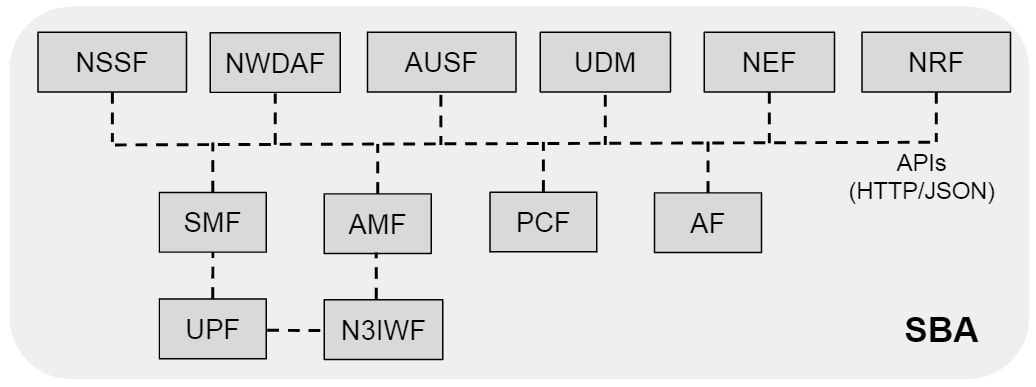
\includegraphics[width=1\textwidth]{TG1/Images/Core5G.png}
    \captionsource{Core 5G software components.}{\cite{Cardoso2020}, p. 15}
    \label{fig:5Gcore}
\end{figure}

\subsubsection{Protocolos NAS, NGAP e PDU}

Os protocolos \textit{Non-Access Stratum} (NAS), \textit{NG Application Protocol} (NGAP) e \textit{Protocol Data Unit} (PDU) são essenciais para a comunicação entre o núcleo da rede, a RAN e o UE. 

O protocolo NAS é usado para fazer a comunicação entre o UE e a função do núcleo AMF, tanto para dispositivos 3GPP quanto nao-3GPP. As principais funções do protocolo NAS são suporte a mobilidade do equipamento de usuário, incluindo procedimentos como autenticação, identificação e atualização das configurações genéricas do UE. Também é responsável por suportar os procedimentos de gerenciamento de sessões, para estabelecer e manter a conexão de dados entre o UE e a rede de dados \cite{3gpp.24.501}. Esse protocolo também é o responsável por fazer a autenticação e gerenciar a conexão da RAN com o núcleo da rede.

O protocolo NGAP é o protocolo padrão para a comunicação do plano de controle entre a RAN e o núcleo da rede. Sendo assim, o NGAP suporta os procedimentos de gerenciamento de interfaces, transporte das mensagens do protocolo NAS, gerenciamento de contexto do UE e das sessões de PDU. O gerenciamento de interfaces é o responsável por estabelecer e manter a conexão entre os componentes do núcleo da rede, onde as mensagens dos protocolos NAS e NGAP são transportados. O Protocolo NGAP é responsável por encapsular e transportar as mensagens NAS, provindas do UE, entre a RAN e o AMF. O gerenciamento de contexto do UE provê informações dos UEs para a RAN, como informações de segurança, lista de restrições de mobilidade e capacidade do rádio do UE. O gerenciamento das sessões de PDU é responsável por gerenciar as sessões de PDU entre o núcleo da rede e a RAN, estabelecendo a interface de rádio utilizada para tráfego de controle e dados dos UEs \cite{3gpp.38.413}.

O protocolo PDU é responsável pelo tráfego de dados do plano de usuário da rede, encapsulando os pacotes de dados sobre o protocolo de rede \textit{User Datagram Protocol} (UDP) \cite{3gpp.38.415}.

\subsubsection{Principais componentes da Rede 5G}

Dentro do núcleo da rede, os componentes AMF, SMF e UPF são os responsáveis por gerenciar todo o tráfego de informações provindos da RAN. O AMF é a porta de entrada do núcleo da rede em relação ao plano de controle. Sendo assim, todo o tráfego utilizando-se os protocolos NAS e NGAP provindos da RAN é direcionado para essa função do núcleo da rede.
Quando uma nova RAN inicia o processo de conexão com um núcleo existente, a autenticação e o estabelecimento da conexão é feito através de mensagens trocadas utilizando-se o protocolo NAS entre a RAN e o AMF. Após estabelecida a conexão, uma mensagem é enviada da RAN para o SMF, indiretamente através do AMF, utilizando-se o protocolo NAS, para que o SMF tenha conhecimento da RAN e possa gerenciar sua sessão.

Estando a RAN operacional, dispositivos 3GPP e não-3GPP dentro da área de cobertura da antena poderão iniciar sua conexão com essa rede 5G. Um dispositivo 3GPP, ao iniciar a conexão com essa rede 5G, troca mensagens com a RAN através do protocolo NAS. A RAN encapsula essas mensagens para o protocolo NGAP e encaminha para o núcleo da rede. O AMF, comunicando-se com os demais componentes da rede, autentica o UE através de um fluxo de informações definido na \textit{Release 15} do 3GPP \cite{3gpp.29.509}. Após concluir a autenticação do UE, o SMF se torna o responsável por gerenciar a sessão do equipamento de usuário. Um fluxo de dados PDU é estabelecido entre o UE e a função do núcleo UPF, que é responsável por gerenciar e encaminhar os pacotes de dados provindos dos UEs.

O UPF é a função do núcleo da rede 5G responsável por ser o ponto de conexão do núcleo da rede com qualquer rede externa. É o UPF que encaminha os pacotes de dados provindos do UE através do protocolo PDU para a rede externa, sendo o responsável pelo roteamento de pacotes entre a rede externa e os diversos UEs conectados nessa rede 5G, além de coletar as métricas da rede que serão usadas na função NWDAF.

A Figura \ref{fig:5Gprotocols} representa a arquitetura de uma rede 5G, exibindo os protocolos NAS, NGAP e PDU entre o equipamento de usuário, a RAN e o núcleo da rede.

\begin{figure}
    \centering
    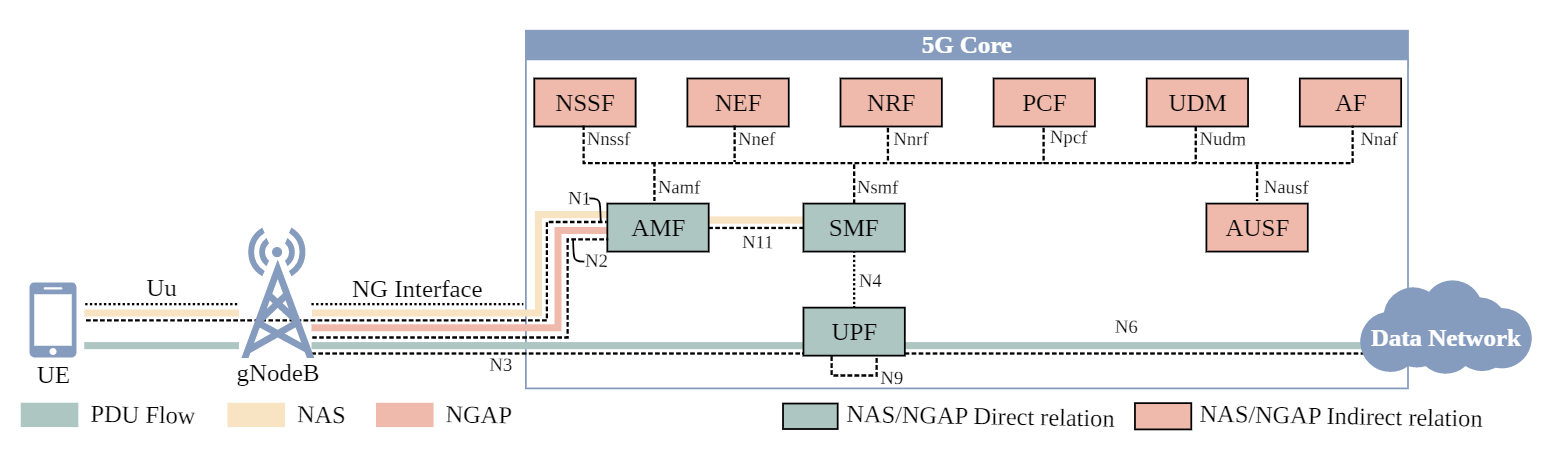
\includegraphics[width=1\textwidth]{TG1/Images/5GSystemProtocols.png}
    \captionsource{5G Core (5GC) Service-based Architecture (SBA).}{\cite{Dominato2021}, p. 3}
    \label{fig:5Gprotocols}
\end{figure}

\subsection{Testes em rede móveis definidas por software}

Segundo \cite{Bertolino2003}, "teste de software consiste na verificação dinâmica do comportamento de um programa em um conjunto finito de casos de teste, adequadamente selecionados do domínio de execuções geralmente infinitas, em relação ao comportamento esperado especificado".

Com relação ao comportamento das redes sem fios implementadas em software, é importante executar testes para que se possa garantir que o funcionamento da rede esteja dentro do esperado.
Dentre os tipos de testes que podem ser executados em cima de implementações de redes 5G \textit{open source}, os que se destacam são os testes de conformidade, robustez e desempenho, como descrito em \cite{Dominato2021} e \cite{Zhang2019ASO}.

\subsubsection{Testes de Conformidade}

Teste de conformidade se define como a atividade de teste realizada com o objetivo de verificar as capacidades e o comportamento de uma implementação em teste em reação aos requisitos de conformidade fornecidos no padrão de protocolo, de acordo com \cite{Sarikaya1989}.
Os resultados dos testes de conformidade são do tipo lógico, sendo verdadeiro no caso onde a implementação em teste seja aprovada no teste e falso no caso contrário.
Dessa forma, o uso de testes de conformidade em redes 5G são importantes para verificar se a implementação da rede móvel se comporta de acordo com a especificação da 3GPP em casos onde o equipamento de usuário execute corretamente as operações descritas.

\cite{Rayner1987} divide o grupo de testes de conformidade em quatro categorias, sendo elas testes básicos de interconexão, testes de capacidade, testes de comportamento e testes de resolução de conformidade.
Os testes básicos de interconexão são feitos para detectar quaisquer casos graves de não conformidade com a especificação do sistema.
Os testes de capacidade verificam se as capacidades observáveis da implementação em teste estão de acordo com os requisitos de conformidade estática da especificação.
Os testes de comportamento verificam a implementação em teste da forma mais abrangente possível para ver se a implementação está de acordo com os requisitos de conformidade dinâmicos da especificação.
Os testes de resolução de conformidade testam em profundidade requisitos específicos na implementação em teste, verificando se a implementação se comporta exatamente como a especificação destes requisitos.

\subsubsection{Testes de Robustez}

Segundo \cite{IEEE.Standard.Glossary}, robustez é definida como "o grau em que um sistema ou componente pode funcionar corretamente na presença de entradas inválidas ou condições ambientais estressantes".
Os resultados dos testes de robustez também são do tipo lógico, sendo verdadeiro no caso onde a implementação em teste seja aprovada no teste e falso no caso contrário.
Sendo assim, o teste de robustez no núcleo de redes móveis verifica o comportamento da rede em situações atípicas e \cite{Dominato2021} divide o grupo de testes de robustez em um subgrupo de testes, que envolve testes de registro, de autenticação e de segurança, além de testes específicos para cada protocolo e função de rede do núcleo.

\subsubsection{Testes de Desempenho}

Os testes de desempenho são importantes para validar o funcionamento da rede em uma carga alta de trabalho, o que representa uma situação de sobrecarga de uso da rede, o que pode causar mal funcionamento da rede e, em situações mais críticas, uma interrupção total do serviço

\textcolor{red}{ToDo}

\textbf{Buscar definições de teste de desempenho (tem aquele artigo sobre MQTT)}

\textbf{Explicar as métricas relacionadas com testes de desempenho e porque elas são importantes}

\textcolor{red}{Falar sobre métricas de latência, perda de pacotes, uso de CPU e tempo de execução}

---------------------------------------------------

\textcolor{red}{\textbf{ToDo: Referenciar os artigos usados.}}




\section{Trabalhos relacionados}
Nesta seção serão analisados alguns estudos publicados com relação a testes em redes móveis.
A Tabela \ref{tab:related-works} apresenta um resumo do estudo realizado de trabalhos relacionados apresentados nesta seção.

\subsection{\textit{Tutorial on communication between access networks and the 5G core}}

O estudo publicado por \cite{Dominato2021} cria uma prova de conceito de uma aplicação para testar núcleos \textit{open source} de rede 5G.
Para esse trabalho, foram escolhidos os grupos de testes de conformidade e robustez.
As implementações suportadas por esse testador são \textit{free5GC}, \textit{Open5GS} e \textit{OAI}.

Essa prova de conceito simula uma RAN e um ou mais UEs.
O objetivo do estudo é analisar o comportamento dos diferentes núcleos de rede 5G em dois diferentes cenários. O primeiro cenário foi executando ações de acordo com o que foi especificado pela 3GPP, através de testes de conformidade. O Segundo cenário foi a execução de ações onde informações inválidas foram informadas, forçando o núcleo da rede a contornar essa situação de acordo com o especificado, o que representa os testes de robustez.

Em relação aos testes de conformidade, foram executados 11 diferentes testes, sendo eles teste de registro, autenticação primária e acordo de chave, identificação, transporte, modo de segurança, atualização de configuração genérica do UE, gerenciamento de sessão, gerenciamento de interface, transporte de mensagens NAS, gerenciamento de contexto do UE e gerenciamento de sessão do PDU.
Foi utilizada a \textit{Release 16} do 3GPP como base para a execução dos testes.
O núcleo \textit{Open5GS} foi aprovado em todos os testes de conformidade, enquanto que o \textit{OAI} e o \textit{free5GC} não responderam de acordo com a especificação no teste de atualização de configuração genérica do UE.

Em relação aos testes de robustez, 7 testes foram executados, sendo eles teste de registro, autenticação, segurança, seleção SMF, seleção UPF, validação do fluxo NAS e gerenciamento de interface.
No teste de registro, dois casos foram avaliados, onde o equipamento de usuário enviou uma requisição de registro sem o identificador do equipamento, que é um campo mandatório e o envio da requisição com as informações criptografadas. Nesse teste, apenas o núcleo \textit{Open5GS} respondeu as requisições de acordo com a especificação.
No teste de autenticação, foram realizadas duas operações incorretas, o primeiro teste foi realizado enviando informações inválidas como resposta no fluxo de autenticação, enquanto que o segundo teste foi forçando uma falha de sincronização entre o núcleo e o UE. Nesse teste, todos os núcleos testados responderam de acordo com a especificação da 3GPP.
Para o teste de segurança, foram testadas duas configurações de segurança inválidas, sendo elas responder a uma solicitação de segurança sem enviar um parâmetro obrigatório na resposta e responder a solicitação sem retransmitir as informações de segurança da requisição. Nesse teste, nenhum dos núcleos avaliados respondeu de acordo com a especificação.
Os teste de seleção SMF e seleção UPF representam um equipamento de usuário fazendo uma requisição para estabelecer um fluxo PDU, porém enviando informações mandatórias inválidas. No teste de seleção SMF apenas o \textit{free5GC} se comportou de forma esperada. Todavia, no teste de seleção UPF, todos os núcleos testados se comportaram de acordo com o esperado.
O teste de validação do fluxo NAS visa verificar se o núcleo da rede se comporta da forma esperada caso a requisição de estabelecimento de sessão PDU seja realizada enviando-se as informações necessárias em uma ordem incorreta. Nesse teste, os núcleos \textit{free5GC} e \textit{Open5GS} se comportaram de acordo com a especificação.
Por fim, o teste de gerenciamento de interface simula o registro de uma nova RAN na rede 5G, porém enviando informações inválidas para o AMF, o qual deve rejeitar essa requisição. Apenas os núcleos \textit{free5GC} e \textit{Open5GS} se comportaram de acordo com a especificação.

O estudo considera que todos os núcleos testados obtiveram um desempenho satisfatório para a operação dentro da normalidade. Entretanto, dentre os três núcleos analisados, o \textit{OAI} foi considerado pelos autores do artigo como o núcleo com a implementação menos madura até o momento da publicação.

Os testes realizados no artigo de Dominato et al. são de extrema importância para avaliar o funcionamento de um núcleo de rede 5G.
Como descrito brevemente no artigo, essa implementação de prova de conceito também suporta a realização de um teste onde múltiplos equipamentos de usuário são conectados no núcleo da rede em forma de fila (realizando uma conexão por vez), afim de avaliar se a implementação em teste do núcleo da rede se comporta de acordo com a especificação em casos onde existam diversos UE conectados na rede.
Entretanto, não foram executados testes para comparar o desempenho dessas implementações de núcleo em casos onde uma grande quantidade de UEs se conectem ao núcleo de forma paralela, onde múltiplos equipamentos de usuário façam requisições de registro e autenticação em um curto intervalo de tempo.
Esse teste é importante para avaliar qual implementação possui a melhor performance em casos de alta carga de trabalho.


\textbf{Reproduzir Figura 2 do artigo do Cristiano, explicando os detalhes do core e os protocolos. Usar esses passos para detalhar os componentes (APIs, protocolos...)} \textcolor{red}{Já adicionei ela na seção passada...}

\subsection{\textit{Realizing 5G Network Slicing Provisioning with Open Source Software}}

O artigo de \cite{Lee2021} trata sobre fatiamentos de rede 5G utilizando-se da implementação \textit{open source free5GC} do núcleo de rede 5G.
A ideia de fatiar uma rede permite criar múltiplas redes lógicas sobre uma única rede física e cada rede lógica tendo suas próprias funções de rede e configurações.
Lee et al. executa cinco experimentos, em duas categorias distintas de testes. Primeiramente, o autor executa um experimento de conformidade, verificando se o fatiamento da rede 5G está de ocorrendo conforme o especificado. Após, são executados quatro experimentos medindo o desempenho do núcleo dessa implementação de rede 5G utilizando-se do fatiamento de rede.

O primeiro experimento executado pelo autor tem como objetivo verificar se os pacotes de dados trafegam por todos os nós na ordem correta, conforme a especificação.
Para isso, o autor utiliza de ferramentas de análise de rede, como o \textit{tcpdump}\footnote{\url{https://www.tcpdump.org}}.
O teste foi bem sucedido, permitindo que os testes de desempenho pudessem ser realizados.

O Segundo teste teve como objetivo medir a qualidade da rede utilizando-se de aplicações específicas para sobrecarregar a rede de dados e medir a vazão da rede 5G.
O terceiro experimento visou medir o desempenho das operações de fatiamento de rede simulando um ambiente de banda larga móvel melhorada, onde o UE executa serviços que geram um alto tráfego de dados na rede.
Nesse experimento, foi observado o tráfego de dados em cada dispositivo e fatia da rede.

O quarto experimento simulou uma rede de sensores, onde diversos dispositivos IoT publicaram informações através do protocolo Message Queuing Telemetry Transport (MQTT)\footnote{\url{https://mqtt.org}} e diversas aplicações se inscreveram para receber as mensagens enviadas.
Foram coletadas métricas de latência, perda de pacotes, uso de CPU e tempo de execução de execuções do experimento variando-se a quantidade de dispositivos se publicando e aplicações se inscrevendo.
Constatou-se que a latência aumentava gradativamente a cada aumento na quantidade de conexões, assim como em certo momento houve perda de pacotes devido a sobrecarga da rede.

O quinto experimento consistiu em criar fatias de rede variando-se a quantidade de funções de rede.
O objetivo desse experimento foi simular serviços de diferentes complexidades, medindo-se a latência gerada ao adicionar mais funções de rede.

Os experimentos executador por Lee et al. são muito importantes para analisar como a sobrecarga de redes móveis afeta o desempenho de redes 5G fatiadas.
Entretanto, esse artigo está realizando os experimentos sobre o plano de usuário da rede, não levando em consideração o quanto o plano de controle da rede foi afetado.

\subsection{\textcolor{red}{ToDo: Falar de outros artigos}}



\begin{table}[]
\centering
\caption{Tabela comparando os trabalhos relacionados}
\label{tab:related-works}
\begin{tabular}{llll}
\hline
\textbf{Autor} & \textbf{Tipos de teste} & \textbf{\begin{tabular}[c]{@{}l@{}}Implementações\\ testadas\end{tabular}} & \textbf{Protocolos testados} \\ \hline
\cite{Dominato2021} & \begin{tabular}[c]{@{}l@{}}Conformidade\\ e robustez\end{tabular} & \textit{\begin{tabular}[c]{@{}l@{}}free5GC, Open5GS\\ e OAI\end{tabular}} & NAS e NGAP \\ \hline
\cite{Lee2021} & \begin{tabular}[c]{@{}l@{}}Conformidade\\ e desempenho\end{tabular} & \textit{free5GC} & Fluxo PDU \\ \hline
\end{tabular}
\end{table}

\section{Método}
Nesta seção, será explicado como pretende-se desenvolver o módulo de teste de performance que vai ser acoplado no my5G-RAN Tester\footnote{\url{https://github.com/my5G/my5G-RANTester}}.
Com o intuito de avaliar o comportamento das diferentes implementações \textit{open source} de núcleo 5G para execução dos procedimentos em escala e utilizando-se como base a prova de conceito do trabalho de \cite{Dominato2021}, propõe-se desenvolver uma extensão para a aplicação my5G-RANTester.
Uma arquitetura em alto nível da aplicação a ser desenvolvida pode ser vista na Figura \ref{fig:tester_arch}.

\begin{figure}[!ht]
    \centering
    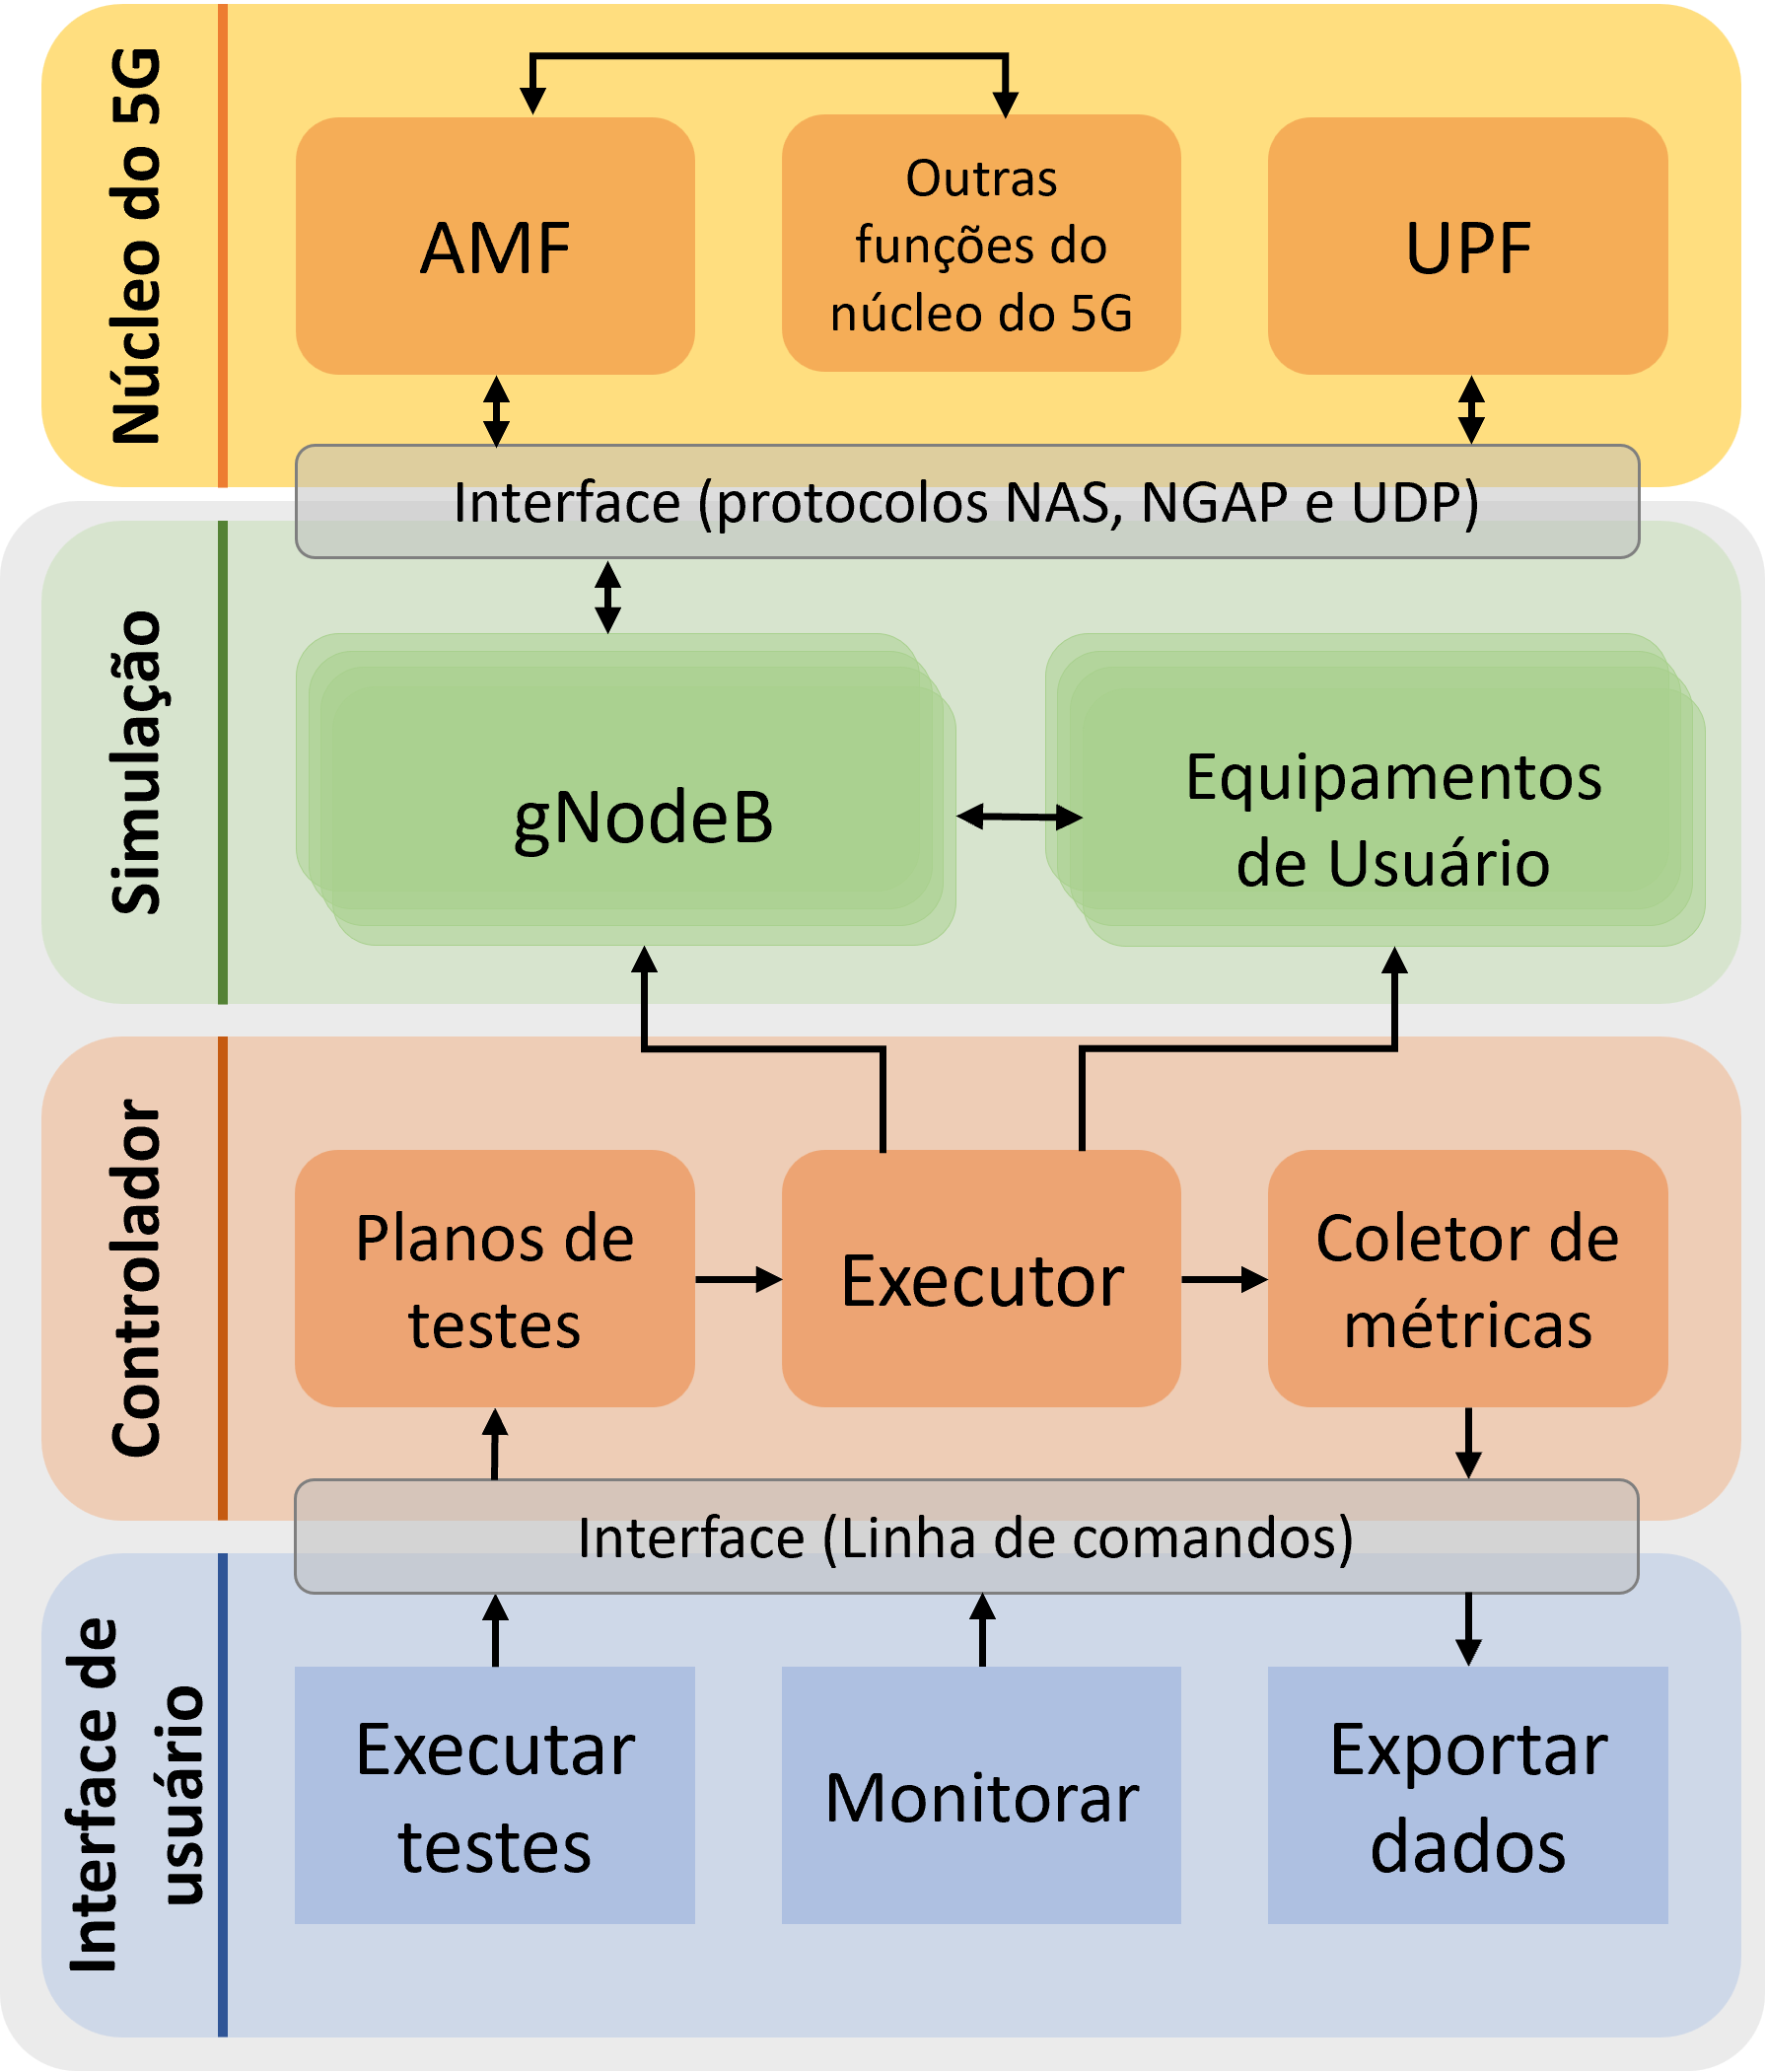
\includegraphics[width=0.6\textwidth]{TG1/Images/TesterArchtectureV2.png}
    \caption{Arquitetura do trabalho}
    \label{fig:tester_arch}
\end{figure}

A camada superior da Figura \ref{fig:tester_arch} representa o núcleo da rede a ser testado. O núcleo em teste implementa uma interface de comunicação que aceita chamadas para a função AMF utilizando-se os protocolos NAS e NGAP. Essa interface também utiliza o protocolo UDP para a comunicação com a função UPF, responsável pelo plano de usuário.

A prova de conceito implementa as três camadas inferiores, sendo elas as camadas de Simulação, do Controlador e da Interface de usuário.
A camada de Simulação irá simular o comportamento de uma ou mais gNodeB e de um ou mais equipamentos de usuário.
Nessa camada, a diferença entre a implementação feita no trabalho de \cite{Dominato2021} e o que será feito no presente trabalho é a capacidade de simular múltiplas gNodeB e UEs simultaneamente, com o intuito de validar a performance de cada implementação de núcleo da rede.

A camada do Controlador é a principal camada no funcionamento do testador. Essa camada recebe os comandos do usuário através de uma interface que define qual teste será executado, controla a camada acima e faz a coleta e o armazenamento das métricas do experimento.
Os planos de testes representam os testes em si que serão escolhidos para serem executados. O Executor recebe as informações do teste e configura as gNodeB e os UEs e envia as métricas para o Coletor de métricas, que irá armazená-las para futuros usos.

Por fim, a camada da Interface de usuário permitirá a execução e o monitoramento dos testes, além de exportar as métricas armazenadas na camada acima. É com essa camada que o usuário do testador irá interagir através de parâmetros enviados por uma linha de comandos a ser executada no ambiente de testes.

A implementação a ser usada como base é feita na linguagem \textit{Go}, criada pela Google em 2009\footnote{https://go.dev/}. O objetivo desse trabalho é estender o testador existente, adicionando a funcionalidade de testes de desempenho.
Para analisar o desempenho das implementações \textit{open source} de núcleos 5G, as métricas a serem coletadas são latência, perda de pacotes da rede e uso de processador e memória RAM da máquina usada para realizar os testes.

\begin{table}[]
\centering
\caption{Configuração da máquina de testes}
\label{tab:vm-config}
\begin{tabular}{lr}
\hline
 & \multicolumn{1}{c}{\textbf{Máquina Virtual}} \\ \hline
\textbf{CPU} & \begin{tabular}[c]{@{}r@{}}Intel Core i9 12900\\ @ 2.4 GHz e 16 núcleos\end{tabular} \\ \hline
\textbf{Memória RAM} & 32 GB DDR5-4800 \\ \hline
\textbf{Armazenamento} & SSD M.2 128 GB NVMe \\ \hline
\end{tabular}
\end{table}

Pretende-se aplicar os testes de desempenho sobre os núcleos \textit{free5GC}, \textit{Open5GS} e \textit{OpenAirInterface}. Os testes serão executados em uma máquina virtual rodando o sistema operacional Ubuntu 20.04 LTS com as seguintes configurações de hardware: processador Intel Core i9 12900, contendo 16 núcleos e 32 GB de memória RAM dedicados, além de 128 GB de armazenamento em um SSD M.2 NVMe. Ao utilizar-se equipamentos de alto desempenho, pretende-se extrair o máximo desempenho dos núcleos de rede 5G, permitindo a conexão de múltiplos equipamentos de usuários e gNodeB e avaliando o comportamento desses núcleos nessa situação. A Tabela \ref{tab:vm-config} exibe o hardware a ser utilizado nos testes.


\section{Proposed schedule}
Para a segunda parte do Trabalho de Graduação (TG2), pretende-se realizar as seguintes tarefas:

\begin{enumerate}
    \item{Estudar a linguagem de programação \textit{Go}.}
    \item{Estudar a implementação do testador de \cite{Dominato2021}.}
    \item{Implementar a extensão do testador para a realização de testes de desempenho.}
    \item{Analisar os resultados obtidos nos testes.}
    \item{Escrever o texto para o TG2.}
    \item{Apresentar o TG2.}
\end{enumerate}

O cronograma de execução das tarefas está disponível na Tabela \ref{tab:cronograma-tg2}.

\begin{table}[!ht]
\centering
\caption{Cronograma de tarefas estipulado para o TG2}
\label{tab:cronograma-tg2}
\begin{tabular}{cccccccc}
\hline
\textbf{Tarefa} & \textbf{Abr} & \textbf{Mai} & \textbf{Jun} & \textbf{Jul} & \textbf{Ago} & \textbf{Set} & \textbf{Out} \\ \hline
\textbf{1} & X & X &  &  &  &  &  \\ \hline
\textbf{2} & X & X &  &  &  &  &  \\ \hline
\textbf{3} &  &  & X & X &  &  &  \\ \hline
\textbf{4} &  &  &  &  & X &  &  \\ \hline
\textbf{5} &  &  &  & X & X & X &  \\ \hline
\textbf{6} &  &  &  &  &  &  & X \\ \hline
\end{tabular}
\end{table}

\textcolor{red}{ToDo: verificar a forma correta de referenciar sites}

\bibliographystyle{sbc}
\bibliography{references,refs-3gpp,refs-web}

\end{document}
